%++++++++++++++++++++++++++++++++++++++++
% Don't modify this section unless you know what you're doing!
%\documentclass[letterpaper,12pt]{article}
\documentclass[14pt]{extarticle}
%\documentclass[journal, a4paper]{IEEEtran}
\usepackage{tabularx} % extra features for tabular environment
\usepackage{amsmath}  % improve math presentation
\usepackage{graphicx} % takes care of graphic including machinery
\usepackage[margin=1in,letterpaper]{geometry} % decreases margins
\usepackage{cite} % takes care of citations
\usepackage[final]{hyperref} % adds hyper links inside the generated pdf file
\usepackage{mathtext}
\hypersetup{
	colorlinks=true,       % false: boxed links; true: colored links
	linkcolor=blue,        % color of internal links
	citecolor=blue,        % color of links to bibliography
	filecolor=magenta,     % color of file links
	urlcolor=blue         
}
\usepackage{textcomp}
\usepackage{ gensymb }
\usepackage{latexsym}
\usepackage{geometry} % пакет для установки полей
\geometry{top=1.5cm} % отступ сверху
\geometry{bottom=2cm} % отступ снизу
\geometry{left=3cm} % отступ справа
\geometry{right=1cm} % отступ слева
\usepackage{amsfonts}
\newcommand*{\No}{\textnumero}
\renewcommand{\Re}{\mathrm{Re}}
\renewcommand{\Im}{\mathrm{Im}}

\newcommand{\const}{\mathrm{const}}
\newcommand{\arccosh}{\mathrm{arccosh}}
%++++++++++++++++++++++++++++++++++++++++

\usepackage[T2A]{fontenc}
\usepackage[utf8]{inputenc}
\usepackage[english, russian]{babel}

\hypersetup{colorlinks=true, linkcolor=black}
\begin{document}

\begin{center}
	\hfill \break
	\large{МИНОБРНАУКИ РОССИИ}\\
	\footnotesize{ФЕДЕРАЛЬНОЕ ГОСУДАРСТВЕННОЕ БЮДЖЕТНОЕ ОБРАЗОВАТЕЛЬНОЕ УЧРЕЖДЕНИЕ}\\
	\footnotesize{ВЫСШЕГО ПРОФЕССИОНАЛЬНОГО ОБРАЗОВАНИЯ}\\
	\small{\textbf{«ВОРОНЕЖСКИЙ ГОСУДАРСТВЕННЫЙ УНИВЕРСИТЕТ»}}\\
	\hfill \break
	\normalsize{Факультут Компьютерных наук}\\
	\hfill \break
	\normalsize{Кафедра Цифровых технологий}\\
	\hfill\break
	\hfill \break
	\hfill \break
	\hfill \break
	\large{Название}\\
	\hfill \break
	\hfill \break
	\hfill \break
	\normalsize{Дипломная работа\\
		\hfill \break
		02.03.01 Математика и компьютерные науки\\
		\hfill \break
		Распределенные системы и искусственный интеллект}\\
	\hfill \break
	\hfill \break
\end{center}

\hfill \break
\hfill \break

\normalsize{
	\begin{tabular}{cccc}
		Зав. кафедрой & \underline{\hspace{3cm}} &  д-р физ.-мат. наук,  проф. & С.Д. Кургалин \\\\
		Студент & \underline{\hspace{3cm}} & &А.А. Махно \\\\
		Руководитель & \underline{\hspace{3cm}}& канд. физ.-мат. наук, доц. &  А.В. Флегель \\\\
	\end{tabular}
}\\
\hfill \break
\hfill \break
\begin{center} Воронеж 2016 \end{center}
\thispagestyle{empty} % выключаем отображение номера для этой страницы

\newpage	
\tableofcontents
\thispagestyle{empty} % выключаем отображение номера для этой страницы
\newpage	
\section*{Введение}
\addcontentsline{toc}{section}{Введение}
Здесь будет введение
\newpage


\section{Физическая задача}

\begin{equation}\label{eq:input}
M_0(\epsilon, t) = \sqrt{\frac{m}{2\pi i \hbar}}\int_{-\infty}^{0} \frac{e^{i \epsilon (t - t')/\hbar}}{(t - t')^{3/2}} [e^{i S(t,t')/\hbar} - 1]dt'
\end{equation} 

\section{Описание метода перевала} 

Метод перевала применяется для оценки при больших значениях параметра $\lambda$ контурных интегралов вида
\begin{equation}\label{eq:eq6}
F(\lambda) = \int_{C}^{}\phi(t)e^{\lambda f(z)}dz
\end{equation} 
где $f(z)$ и $\phi(z)$ функции, аналитические вдоль линии интегрирования С. Интегралами вида (\ref{eq:eq6}) представляются многие специальные функции, решения дифференциальных уравнений, как обыкновенных, так и с частными производными. Эти интегралы часто встречаются при решении различных задач физики.

Рассмотрим частный случай, а именно - действительные интегралы вида

\begin{equation}\label{eq:eq7}
F(\lambda) = \int_{a}^{b}\phi(t)e^{\lambda f(t)}dt
\end{equation} 

Этот случай был рассмотрен в свое время Лапласом. Идея здесь такая. 

Предположим, что $f(t)$ имеет на отрезке $(a, b)$ один резко выраженный максимум. Чем боьше значение параметра $\lambda$, тем резче выражается этот максимум, и поэтому ясно, что при больших $\lambda$ основный вклад в значение интеграла дает окрестность точки максимума. 

В основе этого метода лежит лемма:

\textit{Лемма \label{lemma:lemma1}}: Пусть дан интеграл

$$
F(\lambda) = \int_{0}^{a}\phi(t)e^{-\lambda t^\alpha}dt \:\:\:\:\:\: (0 < a \le \infty, \alpha>0)
$$
где $\phi(t)$ при $|t|<2h$ представляется сходящимся рядом

$$
\phi(t)=t^\beta(c_0+c_1 t+\dots+c_n t^n+\dots), \; \beta>-1
$$
причем $\int_{0}^{a}|\phi(t)| e^{-\lambda_0 t^\alpha}dt\le M$ для некоторого $\lambda_0$. Тогда имеет место асимптотическое разложение

\begin{equation}\label{eq:eq8}
F(\lambda) \sim \sum_{n=0}^{\infty}\frac{c_n}{\alpha} \Gamma\left(\frac{\beta + n + 1}{\alpha}\right)\lambda^{-\frac{\beta + n + 1}{\alpha}}
\end{equation} 
где $\Gamma$ - гамма-функция Эйлера.

К доказанной лемме сводится оценка интеграла (\ref{eq:eq7})

\textit{Теорема 1\label{th:th1}}. Пусть интеграл (\ref{eq:eq7}) абсолютно сходится для некоторого $\lambda = \lambda_0$, т. е.
$$
\int_{a}^{b} |\phi(t)|e^{\lambda_0 f(t)}dt \le M,
$$
и $f(t)$ достигает своего наибольшего значения во внутренней точке $t_0$ отрезка $(а, b)$, в окрестности $| t - t_0| < \delta$ которой $f(t)$ представляется рядом
$$
f(t)=f(t_0) + a_2(t-t_0)^2+\dots+a_n(t-t_0)^n+\dots \;\; (a_2<0),
$$
причем существует $h > 0$ такое, что вне этой окрестности $f (t_0) — f(t) > h$. Пусть еще функция $t = \psi(\tau)$ определяется в окрестности точки $\tau = 0$ из уравнения $f(t_0) — f(t) = \tau^2$, причем в этой окрестности
\begin{equation}\label{eq:eq9}
\phi[\psi(\tau)]\psi^\prime(\tau) = \sum_{n=0}^{\infty} c_n\tau^n
\end{equation}

Тогда интеграл (\ref{eq:eq7}) имеет асимптотическое разложение
$$
F(\lambda)=\int_{a}^{b}\phi(t)e^{\lambda f(t)}dt \sim e^\lambda f(t_0) \sqrt{\frac{\pi}{\lambda}} \sum_{n=0}^{\infty}\frac{c_2n}{\lambda^n}\frac{(2n)!}{4^n n!}.
$$

Эта теорема относится к случаю, когда наибольшее значение $f(t)$ достигается во внутренней точке отрезка $(а, b)$. 

\textit{Теорема 2\label{th:th2}}. Пусть интеграл (\ref{eq:eq7}) абсолютно сходится для некоторого $\lambda = \lambda_0$ (см теорему 1) и $f(t)$ достигает наибольшего значения в точке $t=a$, аналитична в этой точке ($f^\prime(a) \neq 0$), и существует $h>0$ такое, что $f(a)-f(t)>h$ вне некоторой окрестности точки a. пусть еще функция $t=\psi(t)$ определяется в окрестности точки $\tau=0$ из уравнения $f(a) - f(t) = \tau$, причем в этой окрестности имеет место разложение (\ref{eq:eq9}). Тогда

\begin{equation}\label{eq:eq10}
F(\lambda) = \int_{a}^{b}\phi(t)e^{\lambda f(t)}dt \sim \frac{e^{f(a)}}{\lambda}\sum_{n=0}^{\infty}\frac{n! c_n}{\lambda^n}
\end{equation}

Суть метода перевала состоит в том, что при больших значениях параметра $\lambda$ величина интеграла

$$
F(\lambda) = \int_{C}^{}\phi(t)e^{\lambda f(z)}dz
$$
в основном определяется тем участком пути интегрирования $C$, на котором $|e^{\lambda f(z)}|=e^{\lambda \Re f(z)}$, т. е. $\Re f(z)$ велика по сравнению со значениями на остальной части $С$. При этом интеграл оценивается тем легче, чем меньше этот участок и чем круче падает величина $\Re f(z)$ В соответствии со сказанным, при применении метода перевала стараются деформировать путь интегрирования С в наиболее удобный путь $\widetilde{C}$, пользуясь тем, что по теореме Коши такая деформация не меняет величины интеграла.\cite{Lavrentyev}

Чтобы уяснить вопрос геометрически, положим $z = х + iy$ и представим
$$
u = \Re f(z)
$$
как поверхность $S$ в пространстве $(х, y, u)$. Так как функция и гармоническая, то $S$ не может иметь точек максимума и минимума, а точки, в которых $f'(z) = 0$, будут для нее точками перевала (седловыми точками, рис. \ref{ris:image2}).

\begin{figure}[h]
	\center{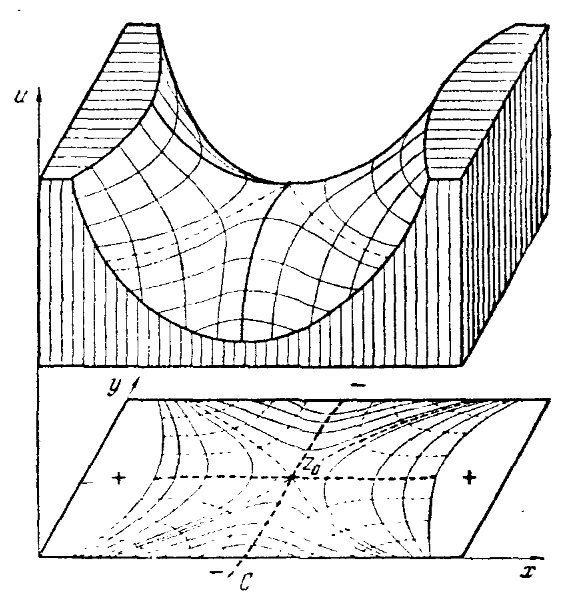
\includegraphics[width=0.3\linewidth]{pic2.png}}
	\caption{Седловые точки}
	\label{ris:image2}
	\end{figure}
	
	Наиболее удобный для оценки путь интегрирования $\widetilde{C}$, в каждой точке должен проходить в направлении наиболее быстрого изменения $\Re f(z)$, а так как функция f(z) аналитическая, то это направление должно совпадать с линией, на которой $\Im f(z) = \const$. 
	
	Также, новый контур $\widetilde{C}$ должен содержать точку $z_0$, в которой $\Re f(z)$ достигает наибольшего значения на $\widetilde{C}$. Покажем для этого случая, что $f^\prime (z_0) = 0$, то есть точка линии $\Im f(z) = \const$, в которой $\Re f (z)$ достигает наибольшего значения, является точкой перевала.
	
	Так и есть, ведь в точке $z_0$, которая является максимумом для $\Re f (z)$ производная $u=0$ вдоль линии $\widetilde{C}$ должна быть равна 0, т. е. $\frac{\partial}{\partial s}\Re f(z)=0$, а так как $\Im f(z) = \const$ на $\widetilde{C}$, то $\frac{\partial}{\partial s} \Im f(z) \equiv = 0$, а значит и 
	
	$$
	f^\prime(z_0) = \frac{\partial}{\partial s} \Re f(z) + i\frac{\partial}{\partial s} \Im f(z) = 0.
	$$ 
	
	\textit{Подведем итоги. Для метода перевала к интегралу (\ref{eq:eq6}) путь интегрирования $С$ следует деформировать в путь $\widetilde{C}$, проходящий через точку перевала $z_0$ и в окрестности этой точки идущий вдоль линии наибольшего ската $\Im f(z) = \const$ (рис. \ref{ris:image2}).}
	
	Есть одно важное обстоятельство, обеспечивающее эффективность применения метода перевала: так как вдоль линии $\widetilde{C}$ имеем $\arg e^{f(z)} = \Im f(z) = \const$, то оценка интеграла (\ref{eq:eq6}) сводится к оценке интеграла от действительной функции, которая может быть проведена по методу Лапласа для интеграла вида (\ref{eq:eq7}).  
	
	Именно это позволяет нам пользоваться полученными результатами теорем 1 и 2. 
	
	Рассмотрим  случай, когда путь интегрирования $С$ можно деформировать в путь $\widetilde{C}$, проходящий через точку перевала $z_0$, где $f^\prime(z_0) = 0$, $f^{\prime\prime}(z_0)\neq0$, и в окрестности $z_0$ совпадающий с линией наибольшего ската $\Im f(z) = \const$, причем на $\widetilde{C}$ вне этой окрестности $\Re f(z) < \Re f(z_0) - h \;(h> 0)$. Кроме того, предположим, что интеграл (\ref{eq:eq6}) абсолютно сходится для достаточно больших значений $\lambda$.
	Тогда образом, оценку интеграла можно провести на основании теоремы 1. Пусть $z = z(t)$ будет уравнение контура $\widetilde{C}$; Тогда,
	
	\begin{equation}\label{eq:eq11}
	F(\lambda) = \int_{C}^{}\phi(z) e^{\lambda f(z)}dz=e^{\lambda i \Im f[z(t)]}\int_{a}^{b}\phi[z(t)]e^{\lambda \Re f[z(t)]}z^{\prime} dt
	\end{equation}
	
	и задача сводится к оценки интеграла вида $\ref{eq:eq7}$ действительной области, разложение для которого уже было получено Лапласом, и имеет вид\cite{Lavrentyev}
	
	$$
	F(\lambda) = \int_{a}^{b}\phi(t)e^{\lambda f(t)}dt \sim \frac{e^{f(a)}}{\lambda}\sum_{n=0}^{\infty}\frac{n! c_n}{\lambda^n}
	$$
	
	Выпишем первый член этого разложения. Обозначим $\phi[z(t)]z^\prime = \widetilde{\phi}(t)$, $\Re f[z(t)] = \widetilde{f}(t)$ и тогда по формуле (\ref{eq:eq10}) получаем:
	
	\begin{equation}\label{eq:eq12}
	\int_{a}^{b} \widetilde{\phi}(t) e^{\lambda \widetilde{f}(t)}dt \sim e^{\lambda \widetilde{f}(t_0)} \sqrt{\frac{\pi}{\lambda}} \widetilde{c_0}
	\end{equation}
	где $\widetilde{c_0}$ - свободный член в разложении функции $\widetilde{\phi}[\widetilde{\psi}(\tau)]\widetilde{\psi^\prime}(\tau)$.
	
	Имеем: $\widetilde{\phi}(t_0) = \phi(z_0) z^\prime (t_0)$, и исходя из того, что $f[z(t)] = \Re f[z(t)]+ i \Im f[z(t)] = \widetilde{f}(t)+\const$ вдоль $\widetilde{C}$, то
	
	\begin{equation}\nonumber
	\widetilde{f}^{\prime\prime} (t_0) = \frac{d^2}{d t^2} f[z(t)]\;|_{t=t_0} = f^{\prime\prime} (z_0) z^{\prime^2} (t_0).
	\end{equation}
	Причем $f^\prime[z(t)] z^{\prime \prime} (t) = 0$ при $t=t_0$. Так как эта величина отрицательна, то представив $z^\prime (t_0) = k e^{i \theta}$, можно записать ее в виде $\widetilde{f}^{\prime\prime}=-|f^{\prime\prime}(z_0)| k^2$. Получаем, что 
	
	\begin{equation}\nonumber
	\widetilde{c}_0=\widetilde{\phi}(t_0) \sqrt{-\frac{2}{\widetilde{f}^{\prime\prime}(z_0)}}= \phi (z_0) e^{i \theta} \sqrt{\frac{2}{|f^{\prime\prime}(z_0)|}}
	\end{equation}
	подставим найденное значение в (\ref{eq:eq12}), а затем в (\ref{eq:eq11}), получаем искомую формулу
	
	\begin{equation}\label{eq:eq13}
	F(\lambda) \sim e^{\lambda f (z_0)}\sqrt{\frac{2\pi}{|f^{\prime \prime} (z_0)|}} \phi(z_0) e^{i \theta} \frac{1}{\sqrt{\lambda}}
	\end{equation}
	
	Как уже много раз говорилось, точка $z_0$ - это точка, где $\Re f(z)$ достигает своего максимального значения. В то же время совершенно обычная ситуация - когда на искомом контуре $\widetilde{C}$ имеется несколько точек перевала, в которых значения $\Re f (z)$ находятся вблизи к наибольшему, то следует взять сумму выражений (\ref{eq:eq13}) по всем этим точками. 
	
	Тот случай, когда контур интегрирования заканчивается в точке перевала $z_0$, аналогичным образом приводится к теореме \ref{th:th2}.
	
	Итак, мы получили рабочую формулу, подставляя в которую составляющие наших искомых функций $\phi (z)$ и $f (z)$, мы должны получать приближенные значения интеграла, когда $\lambda \rightarrow \infty$ 

\newpage
\section{Численное решение}

Выполним численное интегрирование интеграла (\ref{eq:input})

Заметим, что нижний предел интегрирования у нас $-\infty$. Очевидно, что с этими производить вычисления невозможно, но зато наша начальная функция под первым интегралом

$$
A(t) = -c\int_{-\infty}^{t} F(\tau) d\tau
$$

Имеет вид:

\begin{equation}\label{eq:A_eval}
F(t) =  F_0 e^{ -\frac{x^2}{\alpha^2} }  \cos(\omega x)
\end{equation}

и является затухающей. Таким образом, решив уравнение 

$$
|e^{ -\frac{t_b^2}{\alpha^2} }| < \epsilon
$$

на промежутке $[-\infty; 0]$, приближаясь слева, мы получим то самое значение $t_b$, при котором можно не учитывать отрезок интегрирования в связи с достижением необходимой точности.

В этом случае интеграл (\ref{eq:A_eval}) примет вид:

$$\label{eq:easy}
A(t) = -c\int_{t_b}^{t} F(\tau) d\tau
$$

Для вычисления этого интеграла воспользуемся методом интегрирования Гаусса, когда 

$$
\int_{x_1}^{x_2} f(x) dx = \sum_{j=1}^{N} \omega_j f(x_j)
$$

В методе Гаусса точки интегрирования берутся с разными интервалами и при этом имеют различные веса $\omega_i$, характеризующие их вклад в интеграл.

Метод Гаусса также может считать интегралы от неограниченных, быстро затухающий функция. Нам это не потребуется, но в связи с тем, что у нас этот интеграл (\ref{eq:A_eval}) будет входить, далее, в подынтегральные функции, а также с необходимостью на каждом шаге пересчета матричного элемента, менять пределы интегрирования придется использовать адаптивные методы, то есть с переменным шагом. Они не так сложны в реализации, но поскольку вычислений будет очень много, имеет смысл воспользоваться уже готовой библиотекой GNU GSL. 

GNU GSL - Это библиотека, написанная на языке программирования C для численных вычислений в прикладной математике и науке.

Особенности GSL: написана полностью в Стандарте C (также применимое от C++) и основана на использовании заголовочных файлов, определяет новые типы, и структуры данных, у которых нет аналогов в Фортране или C. GSL использует порядок хранения данных на многомерных массивах, который отличается от используемого Фортраном способом. Единственный способ, использование его в Фортране, состоит в том, чтобы записать собственные подпрограммы на C, чтобы обеспечить необходимое соответсвие между типами данных, структурами и соглашениями хранения их для двух языков. Интерфейсный уровень не поставляется с библиотекой. 

Самый главный ее плюс - в скорости вычислений, а также относительная экономия памяти, или же по крайней мере, ограничение ее использования. А также в ней реализовано огромное количество численных методов.

\begin{itemize} 
	\item Базовые математические функции
	\item Комплексные числа
	\item Специальные функции
	\item Вектора и матрицы
	\item Комбинаторика
	\item Сортировка
	\item Линейная алгебра
	\item БПФ
	\item Численно интегрирование (основанное на QUADPACK)
	\item Поиск корней уравнений
	\item и т. д.
\end{itemize}

Нас пока что интересует только один из них, а именно $gsl\_integration\_qags$, позволяющий нам интегрировать функцию на отрезке с заданной точностью. 

Стоит отменить, что для первого интеграла (\ref{eq:A_eval}) GSL не смог добиться точности абсолютной ошибки выше $10^{-13}$, а значит, использовать результат в дальнейшем с большей точностью смысла не имеет.

Далее, у нас есть интеграл $\alpha$

\begin{equation}\label{eq:alpha}
	\alpha(\epsilon, t, t') = \frac{|e|}{c} [A_{\tau}(\epsilon) - \frac{1}{(t-')}\int_{t'}^{t}A(\tau) d\tau]
\end{equation}

Который потом будет входить в интеграл 

\begin{equation}\label{eq:s_integrate}
	S(t, t') = -\frac{1}{2m}\int_{t'}^{t} \alpha(\epsilon, t, t')^2 d\epsilon
\end{equation}

Для упрощения вычислений имеет преобразовать функцию (\ref{eq:s_integrate}) к виду

\begin{equation}\label{eq:s_integrate2}
S(t, t') = -\frac{1}{2m}\int_{t'}^{t} A(\tau)^2 d\tau + \frac{1}{2(t'-t)} \int_{t'}^{t}A(\tau) d\tau
\end{equation}

Итак мы получили функцию $S(t, t')$, которая входит в исходный интеграл ($\ref{eq:input}$). Но сложность для вычислений представляет именно последний интеграл $M$. Для его вычисления рассмотрим преобразование Фурье.

Преобразование Фурье анализирует функцию времени (сигнал) в частоты, которые составляют его.

$$\hat{f}(\xi) =\int_{-\infty}^{\infty}f(x)e^{-2\pi ix\xi }\,dx$$

Когда функция и ее преобразование Фурье заменены дискретизированными дубликатами, ее вызывают дискретным преобразованием Фурье (DFT). 

Дискретное преобразование Фурье преобразоует конечную последовательность равномерно распределенных выборок функции в последовательность эквивалентной длины выборки преобразования Фурье дискретного времени (DTFT), которое является комплексной функцией частоты. Интервал, в котором выполняется DTFT, является обратной величиной продолжительности входной последовательности. Обратное DFT - ряд Фурье, использующее выборки DTFT в качестве коэффициентов сложных синусоид на соответствующих частотах DTFT. Поэтому говорят, что DFT является представлением частотной области входной последовательности. Если исходная последовательность охватывает все ненулевые значения функции, ее DTFT непрерывный (и периодический). Если исходная последовательность - один цикл периодической функции, DFT обеспечивает все ненулевые значения одного цикла DTFT.

$$\begin{aligned}X_{k}=\sum _{n=0}^{N-1}x_{n}\cdot e^{-i2\pi kn/N}=\\=\sum _{n=0}^{N-1}x_{n}\cdot [\cos(2\pi kn/N)-i\cdot \sin(2\pi kn/N)],\end{aligned}$$	


DFT стал оплотом числовых вычислений частично из-за очень быстрого алгоритма для вычисления его, что привело к появлению Быстрого преобразования Фурье (FFT).

Алгоритм быстрого преобразования Фурье (FFT) вычисляет дискретное преобразование Фурье (DFT) последовательности или ее инверсию. Анализ Фурье преобразовывает сигнал (часто всего во времени или пространстве) к представлению в частотной области и наоборот. FFT быстро вычисляет такие преобразования, разлагая на множители матрицу DFT в продукт разреженных (главным образом нуль) факторов. В результате это приводит к уменьшению сложности вычислений DFT от $ O (n^ {2})$, который возникает, при обычном применении DFT до $O (n\log n)$, где $ n $  является размером данных.

Быстрые преобразования Фурье широко используются для многих приложений в технике, науке и математике. Основные идеи были популяризированы в 1965, но некоторые алгоритмы были получены уже в 1805. В 1994, Gilbert Strang описал FFT как "самый важный числовой алгоритм нашего времени".

Заметим схожесть интеграла ($\ref{eq:input}$) с общим видом преобразования Фурье

Введем замену $t - t' = \tau$, получаем

\begin{equation}\label{eq:fourier}
	M(t, \xi) = \int_{0}^{\infty}\frac{e^{i\epsilon \tau}}{{\tau}^{3/2}}(e^{i [+ S(t, t-\tau)]/\hbar} - 1) d\tau\\ 
\end{equation}
$$\hat{F}(\xi) = \int_{-\infty}^{\infty}e^{i\xi \tau} F(\tau) d\tau $$

Для дискретного преобразования Фурье разницы между нашими пределами не будет, так как функция будет определена только на отрезке [0; $t_{end}$].
То есть интегрирование можно ускорить, использовав не стандартные методы интегрирования, а используя дискретное преобразование Фурье. Или же быстрое преобразование Фурье, что будет еще лучшим решением.

Для этого воспользуемся библиотекой FFTW.

Самое Быстрое преобразование Фурье на Западе (FFTW) является библиотекой программного обеспечения для вычислений дискретных преобразований Фурье (DFTs), разработанный Matteo Frigo и Steven G. Johnson в Массачусетском технологическом институте.

FFTW известен как самая быстрая реализация бесплатного программного обеспечения алгоритма Быстрого преобразования Фурье (FFT) (по регулярными сравнительными тестами). Этот алгоритм может выполнить дискретное преобразование Фурье от прсоедовательности со сложным знаком произвольного размера, и размерности в $O (n log n)$, время.

Это делается, поддерживая множество различных алгоритмов, и выбирая один (определенное разложение преобразования в менее сложные преобразования), который оценивают, чтобы быть приоритетным при аналогичных Условия. Это работает лучше всего над массивами размеров с небольшими простыми элементами (оптимальные), и массивами с большими начальными элементами, являющимися худшим случаем (но сложность остается все еще $O (n, log n)$). Разложение преобразовывает алгоритм дискретного преобразования Фурье в алгоритм с  меньшим числом преобразований, (выбор идет среди нескольких вариантов Cooley–Tukey FFT алгоритмов) (соответствующий различным факторизациям и/или различным образцам доступа к памяти), в то время как для больших размеров это используется алгоритм Rader или Bluestein FFT. Как только преобразование было разбито в подпреобразования достаточно меньшей сложности, FFTW использует сложный разбор, разворачивал FFTs для этих небольших размеров, которые были произведены (во время компиляции, не во время выполнения) генерацией кода.

Для достаточно большого количества повторных преобразований выгодно сохранять результаты работы библиотеки для будующего использования алгоритмов на данном размере массива и платформе. Эти результаты, которые авторы именуют как "мудрость", могут быть сохранены в файле или другой последовательности для более позднего использования.

FFTW ограничил поддержку неисправных к текущему времени преобразований (использующий версию MPI). Поэтому переодически приходится переупорядочивать данные.

Именно скорость вычислений - главное что нам потребуется в нашей работе. И, несмотря на то, что повторные вычисления будут запущены на аналогичной архитектуре и, скорее всего, массиве аналогичного размера и вида, использовать сохраненные результаты компиляции прошлого запуска FFTW не имеет смысла, так как компиляция практически не занимает времени, а увеличение сложности вычислений ни коим образом не влияет на усложнение выходного кода библиотеки. Принципиальное усложнение вызывает только увеличение рахмера массива, но основную сложность вычислений составляет не само преобразование Фурье, а получение последоватльности, над которой выполняется преобразование.

Итак, посмотрим еще раз на формулы (\ref{eq:fourier})

Заметим, что если мы возьмем 

$$ 
F(\tau) = \frac{e^{i\epsilon \tau}}{{\tau}^{3/2}}(e^{i [+ S(t, t-\tau)]/\hbar} - 1)
$$

то

$$
\hat{F}(\psi) = \int_{-\infty}^{\infty} e^{i \phi \psi} \frac{e^{i\epsilon \tau}}{{\tau}^{3/2}}(e^{i [+ S(t, t-\tau)]/\hbar} - 1) d\phi
$$

И если положить $\psi = 0$, а также брать отрезок интегрирования от $[0, \infty]$, то $\hat{F}(0)$ будет равно

$$
\hat{F}(0) = M(t, \epsilon)
$$

Это значительно ускорит процесс интегрирования, но слудует понимать, что точек опоры интеграла все равно должно остаться много, чтобы была возможность уловить болльшую часть коллебаний подынтегральой функции.

Таким образом, применение быстрого преобразования Фурье к нашей последовательности с большим количеством точек, и выделение первого элемента получившегося образа дает нам искомую функцию.

Несмотря на эти попытки увеличить производительность, процесс вычисления все еще занимает достаточно долгое время, даже при использовании библиотеки GSL, так как адаптивное интегрирования подынтегральной функции, содержащей в себе еще один интеграл, вызывает некоторые проблеммы точности и на их решение уходит значительная часть вычислительный мощностей. 
Теперь нам есть с чем сравнивать будущее аналитеческое решение
%Который легко интегрируется методом Гаусса.
%



\section{Аналитическое решение}
Получим теперь формулу оценок при помощи метода перевала.

Дана формула (\ref{eq:input})

Часть интеграла с (-1) может быть отброшена, так как (говорилось ранее) основной вклад в интегральную сумму вносят седловые точки. !!!Написать что-нибудь еще!!!

$$
M \sim \int_{-\infty}^{t} \frac{1}{(t-t')^{3/2}} e^{i[\epsilon (t - t') + S(t, t')]/\hbar} dt'
$$

Введем замену $t - t' = \tau$, получаем

$$
M \sim \int_{0}^{\infty}\frac{1}{{\tau}^{3/2}}e^{i [\epsilon \tau + S(t, t-\tau)]/\hbar} d\tau
$$

Если обозначить
$
f(t, \tau) = \epsilon \tau + S(t, t-\tau) 
$ и
$
\phi(\tau) = \frac{1}{{\tau}^{3/2}} 
$

То получим формулу вида

$$
M \sim \int_{0}^{\infty} \phi(\tau) e^{i f(t, \tau)/\hbar} d\tau
$$

Которая совпадает с формулой для Метода Перевала, применимого для интегралов вида (\ref{eq:eq6})

Для нашего случая приближение должно принимать вид:

$$
M_0(\epsilon, t) \simeq \sqrt{\frac{m}{2\pi i \hbar}}\sum_{t0}e^{f(t_0)} \sqrt{-\frac{2}{f''(t_0)}} \phi(t_0)
$$, где $t_0$ - корни уравнения $f'(t) = 0$

Остается только получить формулу для $f''(t)$ и решить уравнение на стационарные точки 

В формулу (\ref{eq:input}) входят некоторые элементы, такие как

$$
S(t, t') = -\frac{1}{2m}\int_{t'}^{t} \alpha(\epsilon, t, t')^2 d\epsilon
$$

$$
\alpha(\epsilon, t, t') = \frac{|e|}{c} [A_{\tau}(\epsilon) - \frac{1}{(t-')}\int_{t'}^{t}A(\tau) d\tau]
$$

$$
A(t) = -c\int_{-\infty}^{t} F(\tau) d\tau
$$

Найдем теперь перевальные точки ($t_0$), дифференцируя по $\tau$

$$
f(t, \tau) = \epsilon \tau + S(t, t-\tau),
$$
$$
f'(t, \tau) = \epsilon + S'(t, t-\tau)
$$
\begin{equation}\label{eq:points}
	f'(t, \tau)=0 => S'(t, t-\tau) = -\epsilon
\end{equation}

С введенной заменой $S$ примет вид

$$
S(t, t-\tau) = -\frac{1}{2m}\int_{t-\tau}^{t} \alpha(\epsilon, t, t-\tau)^2 d\epsilon
$$

Дифференцируя по $\tau$, получаем

$$
S'(t, t-\tau) = -\frac{1}{2m} \alpha(t-\tau, t, t-\tau)^2
$$

Произведем обратную замену $t_0 = t-\tau$ и с учетом того, что $S' = -\epsilon$ (\ref{eq:points}), получаем явный вид уравнения на стационарные точки:

\begin{equation}\label{eq:solvepoints}
\alpha ^2 (t_0, t, t_0) = 2 \epsilon m
\end{equation}

Теперь найдем $f''(t)$

$$
f''(t) = -\frac{1}{2m}\left[\alpha(t-\tau, t, t-\tau)^2\right]' =
$$

$$
= -\frac{2\alpha(t_0, t, t_0)}{2m} \alpha(t_0, t, t_0)'
$$

Рассмотрим новое $\alpha$

$$
\alpha(t_0, t, t_0) = \frac{|e|}{c} \left[A_{\tau}(t_0) - \frac{1}{(t-t_0)}\int_{t_0}^{t}A(\tau) d\tau\right]
$$

%Продифференцируем первую часть ($A_\tau(\epsilon)$) по $t_0$:

%$$
%A'(t_0) = (-c\int_{-\infty}^{t} F(\tau) d\tau)' =
%$$

%$$
%= cF(t_0)
%$$

%И вторую ($\frac{1}{(t-t_0)}\int_{t_0}^{t}A(\tau) d\tau$):

%$$
%\frac{\partial[\frac{1}{t-t_0}\int_{t_0}^{t}A(\tau)d\tau]}{\partial t_0} = -\frac{1}{(t - t_0)^2} \int_{t_0}^{t}A(\tau)d\tau - A(t_0) \frac{1}{t-t_0}
%$$

Итого, получаем формулу для $F''$ вида

\begin{eqnarray}
	F''(t, t_0) = -\frac{|e|\alpha(t_0, t, t_0)}{m} - \nonumber \\
	& \left[F(t_0) - \frac{1}{(t - t_0)^2} \int_{t_0}^{t}A(\tau)d\tau - A(t_0) \frac{1}{t-t_0} \right] \nonumber
\end{eqnarray}


Обозначим $D = - 2 m F''(t, t_0)$ и $$S^\sim = \epsilon \tau + S(t, t-\tau) = \epsilon(t-t_0) + S(t, t_0)$$

Подставляя в формулу для Метода перевала, получаем:

$$
M_0(\epsilon, t) \simeq \sqrt{\frac{m}{2\pi i \hbar}}\sum_{t_0}\frac{e^{\frac{i}{\hbar}S^\sim(t, t_0)} \sqrt{2m}}{\sqrt{D} (t-t_0)^{3/2}} = \frac{1}{\sqrt{\pi i \hbar}}\sum_{t_0}\frac{me^{\frac{i}{\hbar}S^\sim(t, t_0)} }{\sqrt{D} (t-t_0)^{3/2}}
$$

Видно, что полученная формула не слишком проста на вид. Также перед ее вычислением необходимо решать уравнение на стационарные точки для каждого $t$, что, в общем то, не слишком быстрая операция. Рассмотрим сам процесс решения этих уравнений с точки зрения реализации в программе.

Решаем мы уравнение (\ref{eq:solvepoints}). Корни этого уравнения могут быть, в связи с наличием квадратного корня отрицательного числа, комплексные. В этом случае нужно решать систему ($t = const$):

\begin{eqnarray}
\begin{cases}
	\Re \ \alpha(x+i y, t, x+i y) = 2\epsilon m \nonumber\\
	\Im \ \alpha(x+i y, t, x+i y) = 0 \nonumber
\end{cases}
\end{eqnarray}

Здесь $\epsilon < 0$. Для решения этой систему придется перейти в пространству комплексных чисел и производить интегрирование в нем же, что вызывет определенные трудности. Дело не только в интегрировании (входящем в эти уравнения), а также в поиске множества корней. Основным методом решения уравнений в нескольких измерениях является метод градиентного спуска, то есть для него мы должны описать также производные этих функций. Хотя это не вызывает особых сложностей, проблеммой является именно поиск нескольких корней, так как при использовании этого метода необходимо указать приблизительное положение корня в пространстве, а затем, для остальных корней, совершить оптимальный скачок - переход к следующему корню, но нужно быть уверенным, что во время этого перехода не будет потерян промежуточное решение.
Если же положить $ \epsilon = 0$, то система уравнений примет вид 

\begin{eqnarray}
\begin{cases}
\Re \ \alpha^2(x+i y, t, x+i y) = 0 \nonumber\\
\Im \ \alpha^2(x+i y, t, x+i y) = 0 \nonumber
\end{cases}
\end{eqnarray}

Или 

\begin{equation}
	\alpha(x+i y, t, x+i y) = 0
\end{equation};

Это уравнение намного легче решается, поскольку нас теперь интересует только пространство действительных чисел, на котором кони можно найти методом 

\section*{Заключение}
\addcontentsline{toc}{section}{Заключение}
  

 
\newpage
\bibliographystyle{utf8gost705u}  %% стилевой файл для оформления по ГОСТу
\bibliography{biblio}     %% имя библиографической базы (bib-файла) 
\end{document} 